% NOTE TO AIP TYPSETERS: TO CONVERT FROM TWO-COL TO PREPRINT, SWITCH
% COMMENTOUT COMMAND FROM A TO B IE. USE:
%
%%\documentclass[prl,twocolumn,showpacs,twocolumngrid,superbib]{revtex4}
%\documentclass[prl,twocolumn,twocolumngrid,superbib]{revtex4}
%\newcommand{\commentoutB}[1]{}
%\newcommand{\commentoutA}[1]{#1}
%
% INSTEAD OF THE FOLLOWING:
%
\newcommand{\commentoutB}[1]{#1}
\newcommand{\commentoutA}[1]{}
%\documentclass[prl,aps,preprint,showpacs,superbib]{revtex4}
\documentclass[prl,aps,preprint,superbib,12pt]{revtex4}
\usepackage{graphicx}
\usepackage{amsfonts}
\usepackage{amsmath}
\usepackage{bm}
\usepackage{alltt}
\usepackage{fancyhdr}
\newcommand{\bms}[1]{{\boldsymbol #1}}
\renewcommand{\thefootnote}{\fnsymbol{footnote}}

%\draft
%\tighten
\pagestyle{fancy}

\begin{document}

\title{Geometry Optimization of Crystals by the Quasi-\\
       Independent Curvilinear Coordinate Approximation}

\author{K\'aroly N\'emeth\footnotemark[1]}
\author{Matt Challacombe}

\affiliation{Theoretical Division,\\ Los Alamos National Laboratory, \\ Los Alamos, NM 87545, USA}

\date{\today}

\begin{abstract}
This paper presents a performance-assessment 
of the recently developed quasi-independent curvilinear coordinate
approximation (QUICCA) method [K. N\'emeth and M. Challacombe,
J. Chem. Phys. {\bf 121}, 2877, (2004)] for the optimization of crystal 
structures. 
We demonstrate that the concept of quasi-independent
curvilinear coordinates is valid also under periodic boundary 
conditions,
and it leads to highly efficient crystal structure optimizations
as illustrated by a series of test calculations. 
The asessment of QUICCA for the optimization of crystal structures
prooves that QUICCA is a generally applicable algorithm
that is highly efficient for the optimization of both isolated 
molecules and crystals while it preserves an unparalleled robustness 
and simplicity of implementation.
\end{abstract}

%\pacs{31.15.-p,31.15.Ne,02.60.Pn, 45.10.Db, 02.40.Hw} 

\maketitle

\footnotetext[1]{\tt KNemeth@LANL.Gov}

\section{Introduction}
Internal coordinates based on chemical intuition 
are now routinely used in the optimization of 
molecular structures by most standard quantum chemistry program 
packages. Internal coordinates are more advantageous 
for geometry optimization since they exhibit much less 
harmonic and anharmonic vibrational coupling then Cartesians do
\cite{PPulay69,GFogarasi79,GFogarasi92,PPulay77}.
The reduced vibrational coupling allows for much larger steps during the
optimization and results in at least 7-10 times smaller number of 
of optimization steps on small and medium sized molecules
as compared to Cartesian conjugate gradient schemes \cite{TBucko05}.  

Until recently, internal coordinates have been used only to optimize
the structure of isolated molecules.
In recent articles by Kudin {\it et.al.} \cite{KKudin01} and by
Andzelm {\it et.al.} \cite{JAndzelm01} crystal structure optimizations
have been carried out in internal coordinates.
These authors proposed a way
how to build Wilson's B matrix \cite{EWilson55} 
when periodic boundary conditions are present. 
The scheme presented by Kudin {\it et.al.} \cite{KKudin01} allowed for 
the simultaneous relaxation of atomic positions and lattice parameters,
while the one by Andzelm {\it et.al.} \cite{JAndzelm01}  concerned only 
with the relaxation of atomic positions while lattice parameters have 
been fixed. 
An important improvement in the construction of the B-matrix
was very recently carried out by Bu\v{c}ko, Hafner and {\'A}ngy{\'a}n
\cite{TBucko05}.
These authors realized that 
all internal coordinates may have non-vanishing contribution
to the displacement of lattice parameters, and not only those
that cross the boundaries of the central cell. 
In our opinion, the paper of Bu\v{c}ko, Hafner and {\'A}ngy{\'a}n
provides the first complete determination of Wilson's B matrix
for crystals. Their definition of the B matrix will be used through
the present paper. 

In the present article we want to assess the performance of our recently
developed optimization algorithm, the Quasi Independent Curvilinear 
Coordinate Approach (QUICCA) \cite{KNemeth04} 
in crystal structure environment.
QUICCA is based on a radical exploitation of the approximate decoupling
of the harmonic and anharmonic vibrational couplings in
internal coordinate representation.
QUICCA is simple 
to implement, robust and very efficient for isolated molecules while
its computational cost scales linearly with the system-size for each 
optimization step. However, nothing is known yet about the 
applicability of QUICCA for crystals. In crystals, coupling effects
may be very different from the ones in isolated molecules. If QUICCA
works similarly well for crystals as it does for isolated molecules
it can be used as a generally applicable, extremely robust 
internal coordinate optimizer for the optimization of large 
molecules and crystals. 

In the following, we first review the construction of Wilson's B matrix
for crystals (Sec. \ref{crystalBmat}), then the QUICCA algorithm is 
reviewed as applied for crystals (Sec. \ref{QUICCAreview}, 
finally results of test calculations
ranging over a broad class of crystalline systems are presented
(Sec. \ref{ResDissc}). Finally, we conclude the analysis of the results
in that QUICCA is a very efficient method for optimizing both
crystal structures and isolated molecules (Sec. \ref{Conclusions}).

\section{Methodology}
\subsection{Wilson's B matrix for crystals} \label{crystalBmat}
In this section we briefly review how the elements of Wilson's
B matrix can be calculated for crystals. A more detailed discussion 
of this issue can be found in Ref. \onlinecite{TBucko05}.

The independent geometrical variables of a crystal are the 
fractional coordinates, $f_{k}$ and the lattice vectors, $h_{l}$.
The absolute Cartesian position, $r_{k}$ of the $k$-th atom
can be decomposed as a funtion of both the fractional coordinates 
$f_{k}$ of atom $k$ and the lattice vectors:
\begin{equation}
r_{i} = h f_{i} ,
\end{equation}
where the matrix $h$ contains the Cartesian components of the 
$h_{1}$, $h_{2}$ and $h_{3}$ lattice vectors in its 
columns, respectively.

The B matrix for crystals contains the total derivatives 
of internal coordinates with respect to fractional ones
and lattice vectors:
\begin{equation}
B_{ik} = \frac{d \phi_{i}}{d f_{k}} ,
\end{equation}
\begin{equation}
B_{il} = \frac{d \phi_{i}}{d h_{l}} ,
\end{equation}
where $\phi_{i}$ is the $i$-th internal coordinate,
and $B_{ik}$ is a 3-component vector, similar to $f_{k}$ and $h_{l}$.

In order to compute elements of the B matrix of a crystal, the above
expressions must be
related to B matrix elements of isolated molecules. This decomposition
can be done by the application of the chain rule to the above 
total derivatives, which results in
\begin{equation}
B_{ik} =  \frac{\partial \phi_{i}}{\partial r_{k}} h ,
\end{equation}
and 
\begin{equation} \label{Blattice}
B_{il} =  \sum_{m=1}^{4} 
          \frac{\partial \phi_{i}}{\partial r_{m}} f_{ml},
\end{equation}
where $\frac{\partial \phi_{i}}{\partial r_{k}}$ and 
$\frac{\partial \phi_{i}}{\partial r_{m}}$ are row-vectors and contain
the partial derivative of the $i$-th internal coordinate
with respect to the absolute Cartesian positions of 
the $k$-th and $m$-th atoms. $f_{ml}$ represents the
$l$-th component of the fractional coordinates of the $m$-th atom.
Note, that $f_{ml}$ can be greater then $1$ if the $m$-th atom is not 
in the central cell.
The partial derivatives $\frac{\partial \phi_{i}}{\partial r_{m}}$ 
are identical
with the B matrix elements of isolated molecules. The summation
in Eq. \ref{Blattice} goes over all atoms that compose $\phi_{i}$,
i.e. in case of primitive internal coordinates over maximum $4$ atoms. 

\subsection{Preparation of gradients}
Our linear scaling electronic structure program, MondoSCF \cite{MondoSCF} provides
the energy gradients on the absolute Cartesian positions, 
$\frac{\partial E}{\partial r_{k}}$, and the total derivatives
of the energy with respect to lattice vector components, 
$\frac{d E}{d h_{l}}$.
To calculate the forces, $\frac{d E}{d \phi_{i}}$, which act on the
internal coordinates, the total derivatives of the energy,
$\frac{d E}{d f_{k}}$ and 
$\frac{d E}{d h_{l}}$ are needed of which $\frac{d E}{d h_{l}}$ is 
given by our electronic stucture code.
$\frac{d E}{d f_{k}}$ can easily be calculated as:
\begin{equation}
\frac{d E}{d f_{k}} = \frac{\partial E}{\partial r_{k}} h .
\end{equation}
For the sake of completeness the relationship between total and
partial derivatives of the energy with respect of the lattice vectors
is defined by
\begin{equation}
\frac{d E}{d h_{l}} = \frac{\partial E}{\partial h_{l}} +
                      \sum_{n=1}^{N_{a}} 
                      \frac{\partial E}{\partial r_{n}} f_{nl} ,
\end{equation}
where $N_{a}$ is the number of atoms in the elementary cell 
\cite{TBucko05}.



\subsection{Coordinate transformations}
Once the B matrix is given, the gradients on the internal coordinates
are calculated by solving 
\begin{equation} \label{solveintcgrads}
B^{t} g_{i} = g_{c} ,
\end{equation}
where the first $3N_{a}$ elements of $g_{c}$ contain 
the $\frac{d E}{d f_{k}}$ gradients and the last $9$ elements contain
the $\frac{d E}{d h_{l}}$ ones and the superscript $t$ means 
transposition.

The coordinate transformations are carried out in a linear scaling 
fashion, as described in Refs. \onlinecite{KNemeth00} and 
\onlinecite{KNemeth01}. It is worth to mention, that the last 9 columns
of the B matrix which refer to lattice derivatives of the internal 
coordinates may be full, as opposed to the first $3N_{a}$ columns 
which are extremely sparse. Even with 9 colums full, the Cholesky
factorization of the $G_{c}=B^{t}B$ matrices can be carried out
in a linear scaling fashion, since the first $3N_{a} \times 3N_{a}$
block of $G_{c}$ preserves its extreme sparsity, similar to the
case of isolated molecules \cite{KNemeth00}.
Thus the solution of Eq. \ref{solveintcgrads} can be carried out 
in a linear scaling fashion also for crystals.
Note that the sparsity in the Cholesky factorization step cannot be
preserved when an alternative solver, based on the $G_{i}=BB^{t}$
matrix is used, thus this latter kind of solver 
is inefficient to carry out
the coordinate transformation for large crystals.

Once predictions are done for improved values of internal coordinates
on the basis of internal coordinate gradients and the QUICCA 
\cite{KNemeth04} algorithm, the new Cartesian coordinates 
are calculated via the iterative back-transformation
as described in Ref. \onlinecite{KNemeth04}, which also scales 
linearly with the system-size. At each step of the iterative 
back-transformation fractional coordinates and lattice vectors
are updated and the corresponding atomic Cartesian coordinates are
generated to determine the updated values of internal coordinates
at an updated lattice structure. The rest of the back-transformation
is the same as what is used for isolated molecules.

\section{Implementation}

\subsection{The QUICCA algorithm for crystals} \label{QUICCAreview}
Details of the QUICCA algorithm for geometry optimization 
of isolated molecules are 
described in our previous paper \cite{KNemeth04}. Here we provide 
only a very brief summary of the most important features of the 
optimizer.
QUICCA is based on the realization of the fact, that internal coordinate
gradients show trends during geometry optimization.
These trends can be formalized by weighted curve fitting for each 
individual internal coordinate, over internal coordinate value and 
gradient data-pairs.
In practice, this curve fitting is most robust with just a line-fit. 
The root of the
fitted curve (line) provides an improved estimate for the minimum
along the internal coordinate. Collectively, these minima determine
the optimization step at the actual geometry.
QUICCA works well, because internal coordinates exhibit  
reduced harmonic and anharmonic vibrational coupling, as
compared to Cartesian ones. Furthermore, the fitting process
has an important averaging effect on the vibrational coupling
that also strongly contributes to the success of QUICCA.
A typical fitting process of a gradient curve is illustrated in 
Fig. \ref{iceIh} on a hydrogen bond of the hexagonal (P63/MMC)
ice structure \cite{AGoto90}.

\begin{figure}[h]
\resizebox*{3.5in}{!}{\includegraphics{IceIhfit.eps}}
\caption{
Progression of gradients on a hydrogen bond coordinate
of the hexagonal ice crystal.
Energies and forces have been obtained by the Hartree-Fock
model in STO-3G basis set.
The optimization was started from the crystallographic structure
\cite{AGoto90}.
The numbers in the picture
indicate the sequence of optimization steps. The dashed line represents
a weighted linear fit, the star the predicted location of the minimum.}
\label{iceIh}
\end{figure}

The only change that our recent implementation of QUICCA contains as 
compared to the formerly described one (Ref. \onlinecite{KNemeth04})
is that merging of the connectivities from recent optimization steps
does not take place any more. Omitting the merger of connectivities
does neither change results on Baker's test set as given 
in Ref. \onlinecite{KNemeth04}, nor decreases efficiency of optimization
on large protein fragments.

\subsection{Data preparation}
At the beginning of the fitting process of QUICCA
Cartesian coordinates of past optimization steps are compared to a
reference geometry and those Cartesian positions of the past 
crystal structures are retrieved that are the closest ones
to the reference geometry. This pre-caution is necessary
to avoid sudden jumps in internal coordinate values due to the
fact that atoms crossed the boundaries of the central cell during 
the optimization.

\subsection{Recognition of the internal coordinates}
The Cartesian central cell is replicated so, that all $27$ 
cells with lattice indices between $-1$ and $+1$ are generated.
Even though a smaller replica of 8 cells, with lattice indices
between $0$ and $1$ contains all necessary local internal coordinates,
we prefer to start from the bigger cell, to avoid fragmentation
of molecules at the boundaries of the central cell.
Then, all internal coordinates are recognized in the supercell
by means of the recognition algorithm described in our previous paper
\cite{KNemeth04}, just as for isolated molecules.
Finally, all internal coordinates will be discarded that do not 
have at least one atom in the central cell. Note that the
result of this procedure may contain symmetry equivalent
internal coordinates, among those internal coordinates that cross
the boundaries of the central cell. In present applications
we did not filter out these equivalent coordinates since their
presence has no major effect on the process of the optimization. 
For each of the symmetry equivalent coordinates the gradient curve
is exactly the same with the same root.

\subsection{Treatment of constraints}
In the presence of constraints, the constraint-space
component of the Cartesian gradients is projected out 
at the beginning of the optimization, as described
in Ref.~\onlinecite{PPulay77}. Gradient based convergence criteria
observe only these purified gradients. This purification 
step is also meant to ensure that gradients on constrained
internal coordinates be zero after the gradient transformation step
(when Cartesian gradients are transformed into internal coordinate
representation, \cite{PPulay77}).

In the rest of the treatment of the constraints, we distinguish
the soft and the hard constraints.
Soft constraints approach their required value during the
optimization process and will be set latest at the end of the
optimization. Most internal coordinate constraints are such
in our implementation. Hard constraints are set to their required
value right at the beginning of the optimization process and keep their
value during the course of the optimization. 
Cartesian constraints and lattice constraints are hard constraints 
in our implementation. 
The application of the soft constraints is
useful in situations when it would be difficult to construct the 
Cartesian coordinates that satisfy the required values of internal 
coordinate constraints {\it prior} to the optimization. 
Thus, the potentially laborous input construction
is saved and all constraints related tasks are passed into the 
optimizer.

Our way of treating hard constraints is similar to Baker's projection
scheme \cite{JBaker96}.
Those coulumns of the $B$ matrix that refer 
to hard constraints are entirely zeroed. 
The zeroing process in the B matrix reflects the simple fact 
that the variation of any internal coordinate may not contain 
contribution from a Cartesian coordinate or lattice parameter 
that is constrained.
Note, that if lattice parameters are constrained, the last 9 columns
of the $B$ matrix ($\frac{d \phi_{i}}{d h_{l}}$) must be trasformed
from lattice-vector representation into lattice-parameter 
representation by using the generalized inverse of the lattice-parameter
Jacobian. This transformation results in 6 columns referring to the 
6 lattice parameters. 
After zeroing the required columns, 
this portion of the $B$ matrix is transformed back into the original
9 columns representation.

The zeroing of the selected colums of $B$ immediately
ensures that during the iterative back-transformation 
\cite{PPulay77} no displacements occure on hard constraints.

Soft constraints will be treated in a slightly different way. 
Baker's projection algorithm recommends to purify each row
of the B-matrix by essentially the same projector that is being used
in the purification of the Cartesian gradients. 
A computationally more efficient formulation of this step for the
gradient transformation looks like
\begin{equation}
g_{i} = B P G_{c}^{-1} P g_{c} ,
\end{equation}
where $P$ is the purification projector that filters out the 
constraint-space component of vectors \cite{PPulay77} and
$G_{c}^{-1}$ is the generalized inverse of $G_{c}=B^{t}B$.
The first step of 
this projection, $g_{c}' = P g_{c}$ is already done at the initial
purification of the Cartesian gradients. The second step would be
$P G_{c}^{-1} g_{c}'$, which we currently skip in our implementation, 
since as the purified Cartesian gradients converge this second
purification step has less and less importance.

The skipping of the second purification step is optional
for the gradient transformation, but it is obligatory for the iterative
back-transformation as the iterative back-transformation is
expected to change the values of soft-constraints and
put them as close as possible to their required (constrained) value.
The required new values of the internal coordinates are constructed
by by the QUICCA algorithm except for the constrained internals,
whose value is determined by the input. The iterative 
back-transformation takes these required values and finds the best fit
in terms of Cartesian coordinates, as described in Refs. 
\onlinecite{PPulay77} and \onlinecite{KNemeth00}.

\subsection{Realization}
The crystal structure optimizer has been implemented in the
MondoSCF suite of linear scaling quantum chemistry codes 
\cite{MondoSCF}, in the object oriented 
FORTRAN-90/95 programming language.
Lattice forces have been calculated analytically, as described in 
Ref.~\cite{CJTymczak04LatF}. Note, that all energies and gradients
have been calculated by means of the gamma point approximation,
i.e. there is no band structure calculation in our treatment.

\section{Results and discussion} \label{ResDissc}
\subsection{The test set}
Our test set of crystal optimizations contains
6 different systems:
Polyethylene, hexagonal boron-nitride , (10,0)carbon-nanotube,
Ice \cite{AGoto90}, 
Quartz \cite{MGTucker01}, 
Sulphure \cite{ACGallacher92}. 
In addition to these structures
we also demonstrate the power of our optimizer
on PETN, a 50 atoms high-explosive \cite{Trotter_1963v16,Conant_1979}
which forms hydrogen-bonded crystals.
Most of the structures were
taken either from the Inorganic Crystal Stuctures Database
(ICSD) \cite{ICSD} or from Cambridge Crystallographic Data Center
\cite{CCDC} and the translationally unique positions were
generated using Mercury \cite{Mercury}. 
In the following subsections input geometries are described that
have been prepared by additional manipulation after 
the primary structure have been downloaded
from the crystallographic data-base.  

\subsubsection{Polyethylene}
The quasi one-dimensional structure of polyethylene has been defined 
by the starting Cartesian coordinate set
\\
{\tt C    0.500   0.500   0.000} \\
{\tt H    0.500   1.300   0.800} \\
{\tt H    0.500   1.300  -0.800} \\
{\tt C    1.500  -0.500   0.000} \\
{\tt H    1.500  -1.300   0.800} \\
{\tt H    1.500  -1.300  -0.800}, \\
with a $2${\AA} long lattice vector along the $X$ axis. 

\subsubsection{Hexagonal boron-nitride}
The two-dimensional hexagonal boron-nitride has been 
defined by the starting fractional coordinates
\\
{\tt B 0.33333333333 0.1666666666 0.0000000000} \\
{\tt N 0.66666666666 0.8400000000 0.0000000000}, \\
and lattice parameters $a=2.420${\AA}, $b=2.420${\AA} and 
$\gamma=120^{\rm o}$.

\subsubsection{(10,0)carbon-nanotube}
In the one-dimensional polymer, (10,0)carbon-nanotube,
all bond-lengths that are parallel to the axis of the
nanotube have been initially $1.480${\AA} long, while those
running perpendicularly to the axis have been $1.402${\AA} long.
The only cell parameter $a$ was initially $a=4.44${\AA}. The
elementary cell contained 40 atoms. These data entirely determine
the structure of the symmetric (10,0)carbon-nanotube.

\subsubsection{Ice}
Hexagonal ice is the most important natural occurance of ice.
Its structure has been taken from the literature \cite{AGoto90}. 
Since the literature provides two equilibrium position
for each hydrogen atoms due to the tunneling of hydrogens in ice,
our starting structure contained the average of these two positions
for each hydrogen atom. The translational elementary cell contains
four water molecules.

\subsection{Results}
Energies and forces have been calculated on the PBE/STO-3G level of 
theory, in the $\Gamma$-point approximation. 
The optimizations have been carried out by means of the
QUICCA method as described above,
simultaneously optimizing atomic positions and lattice vectors,
all geometric parameters have been completely flexible during the 
course of the optimization.
In these optimizations a single
convergence criterium has been used, namely that the maximum
magnitude of both atomic and lattice vector gradients had to be
smaller then 0.0005 a.u. at convergence.
Table \ref{optsteps} shows the number of optimization steps and
the optimum energy. While the first four test systems converged quickly,
quartz and sulphure took substantially more steps to the optimum.
in the case of quartz this is due to a very large structural change,
namely four membered rings have been formed in the optimum structure,
that probably indicates that the small basis applied and maybe 
also the $\Gamma$-point approximation is very inappropriate
for this system. The optimum structure of quartz is shown in
Figure \ref{quartz}.
In the sulphure crystal, the $S_{8}$ rings interact via Van der Waals
interaction and this interaction potential is very flat. One way
to accelerate the optimization of such a shallow potential surface
is to use the so called $5/R$ coordinates instead of the stretches
we have used to optimize inter-ring distances. We plan to compare
these two coordinate sets in a forthcoming study.

\begin{table}[h]
\caption{Optimization results for crystal structures
at the PBE/STO-3G level of theory and in the $\Gamma$-point 
approximation, using the QUICCA algorithm.}
\label{optsteps}
\begin{tabular}{lcr}
\toprule
                       & Number of           & Optimum energy\\
Molecule               & optimization steps  &  (a.u.) \\
\colrule
polyethylene           & 8   &    -77.56774   \\
boron-nitride          & 5   &    -78.41368   \\
(10-0)carbon-nanotube         & 7   &  -1503.75024   \\
ice                    & 15  &   -301.31784   \\
quartz                 & 44  &  -1303.03159   \\
sulphure               & 89  & -12595.53586   \\
\botrule
\end{tabular}
\end{table}

\subsubsection{Convergence of the energies}
As discussed in our previous paper on the QUICCA optimization
algorithm \cite{KNemeth04}, QUICCA converges as a first
order optimization scheme. This convergence feature
is also illustrated in Figures \ref{ch2-energ}-\ref{Sulphure-energ}.

\subsubsection{Convergence of the gradients}
Figures \ref{ch2-grad}-\ref{Sulphure-grad} illustrate the convergence
of the magnitude of maximum atomic and lattice-vector gradients.
The convergence is smooth and rapid in all cases with the exception
of the sulphure crystal, which is due to the shallow van der Waals
potential energy surface between the $S_{8}$ sulphure rings.
Also note that the atomic and the lattice gradient curves run close
to each other which is a sign of balanced optimization
between lattice and atomic posions when simultaneously
optimizing atomic positions and lattice in the QUICCA scheme.

\begin{figure}[h]
\resizebox*{3.5in}{!}{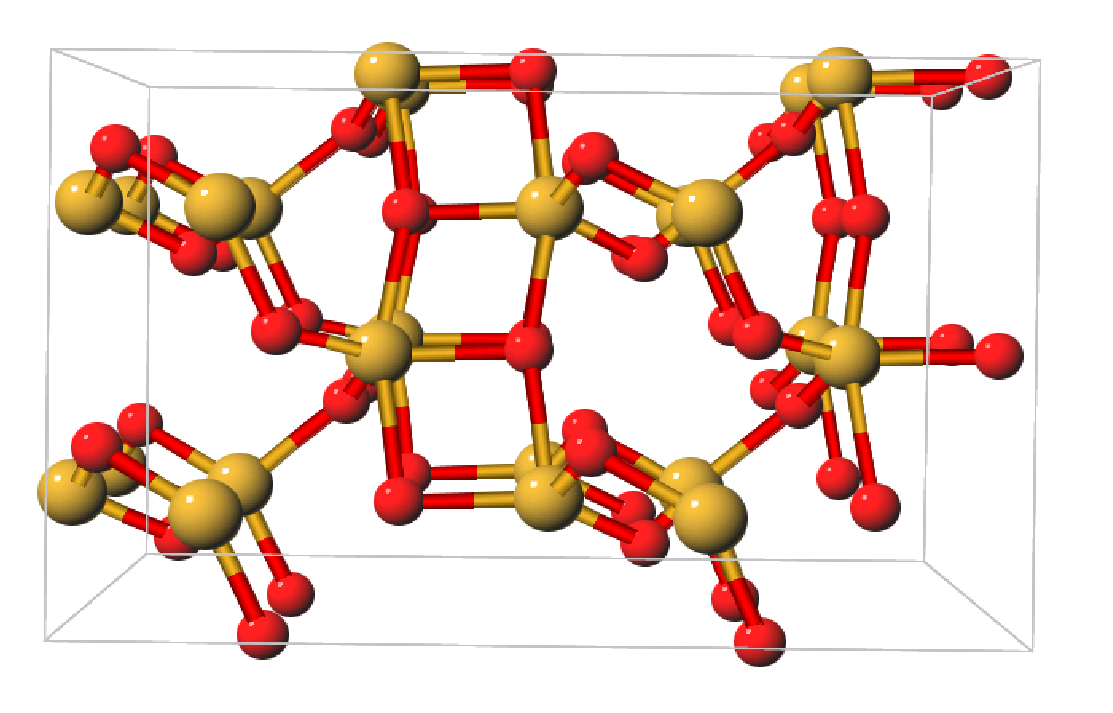
\includegraphics{quartz.eps}}
\caption{The optimum structure of quartz at the PBE/STO-3G
level of theory and in the $\Gamma$-point approximation.}
\label{quartz}
\end{figure}

\begin{figure}[h]
\resizebox*{3.5in}{!}{\includegraphics{ch2-energ.eps}}
\caption{Convergence of the energy during the optimization
of polyethylene.}
\label{ch2-energ}
\end{figure}

\begin{figure}[h]
\resizebox*{3.5in}{!}{\includegraphics{BN1x1-energ.eps}}
\caption{Convergence of the energy during the optimization
of hexagonal boron-nitride.}
\label{BN1x1-energ}
\end{figure}

\begin{figure}[h]
\resizebox*{3.5in}{!}{\includegraphics{NANO-energ.eps}}
\caption{Convergence of the energy during the optimization
of the (10,0)carbon-nanotube.}
\label{NANO-energ}
\end{figure}

\begin{figure}[h]
\resizebox*{3.5in}{!}{\includegraphics{ICE-energ.eps}}
\caption{Convergence of the energy during the optimization
of hexagonal ice.}
\label{ICE-energ}
\end{figure}

\begin{figure}[h]
\resizebox*{3.5in}{!}{\includegraphics{Quartz-energ.eps}}
\caption{Convergence of the energy during the optimization
of quartz.}
\label{Quartz-energ}
\end{figure}

\begin{figure}[h]
\resizebox*{3.5in}{!}{\includegraphics{Sulphure-energ.eps}}
\caption{Convergence of the energy during the optimization
of sulphure.}
\label{Sulphure-energ}
\end{figure}

\begin{figure}[h]
\resizebox*{3.5in}{!}{\includegraphics{ch2-grads.eps}}
\caption{Convergence of the gradients during the optimization 
of polyethylene.}
\label{ch2-grads}
\end{figure}

\begin{figure}[h]
\resizebox*{3.5in}{!}{\includegraphics{BN1x1-grads.eps}}
\caption{Convergence of the gradients during the optimization
of hexagonal boron-nitride.}
\label{BN1x1-grads}
\end{figure}

\begin{figure}[h]
\resizebox*{3.5in}{!}{\includegraphics{NANO-grads.eps}}
\caption{Convergence of the gradients during the optimization
of (10,0)carbon-nanotube.}
\label{NANO-grads}
\end{figure}

\begin{figure}[h]
\resizebox*{3.5in}{!}{\includegraphics{ICE-grads.eps}}
\caption{Convergence of the gradients during the optimization 
of hexagonal ice.}
\label{ICE-grads}
\end{figure}

\begin{figure}[h]
\resizebox*{3.5in}{!}{\includegraphics{Quartz-grads.eps}}
\caption{Convergence of the gradients during the optimization
of quartz.}
\label{Quartz-grads}
\end{figure}

\begin{figure}[h]
\resizebox*{3.5in}{!}{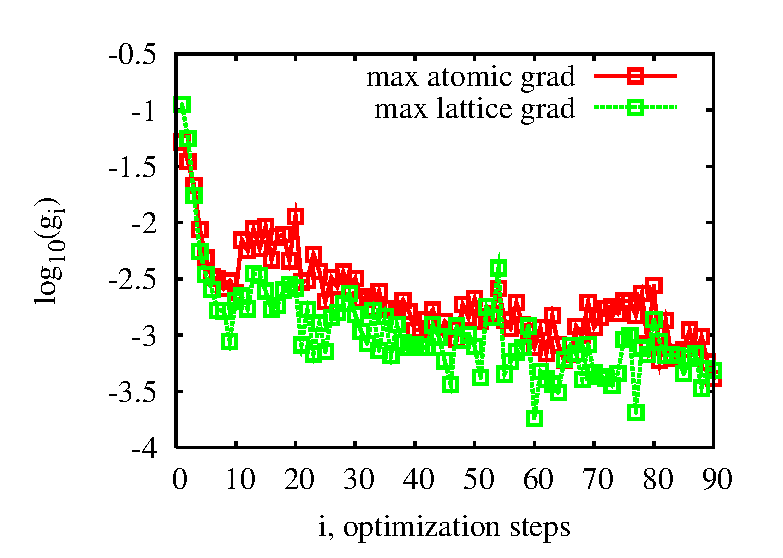
\includegraphics{Sulphure-grads.eps}}
\caption{Convergence of the gradients during the optimization 
of sulphure.}
\label{Sulphure-grads}
\end{figure}

\section{Conclusions} \label{Conclusions}
We have demonstrated that the QUICCA algorithm is an efficient
way to optimize various crystal structures of one, two and three
dimensional periodicity. The crystals of our test set are held
together by either covalent bonds, or hydrogen bonds or even
by van der Waals interactions. Succesful optimizations
have been carried out in every possible dimensionality and crystal types
while fully and simultaneously relaxing all geometric parameters.
This study demonstrates that QUICCA is a robust and generally applicable
optimization algorithm that can be applied both to gas-phase
molecules and periodic systems.

\bibliography{../../Bib/mondo_new}
\end{document}
